\documentclass[a4paper]{article}


\usepackage{alphabeta} 
\usepackage{enumitem} 
\usepackage{mathtools}
\usepackage{amsmath, amssymb} 
\usepackage{amsthm}
\usepackage{cancel} 
\usepackage[margin=0.70in]{geometry} 
\geometry{left=2cm,right=2cm,top=2.4cm,bottom=2.4cm}	%the page geometry as defined, A4=210x297mm
\usepackage{graphicx}
\usepackage{wrapfig}
\usepackage[center]{caption}
\usepackage{textcomp}
\usepackage{tabto}
\usepackage{layout}
\usepackage{bm}
\usepackage{minipage-marginpar}
\usepackage[dvipsnames]{xcolor}
\usepackage{hyperref}
\usepackage{dutchcal}
\usepackage{derivative}
\usepackage{esint}
%\usepackage{biblatex}
\usepackage{subcaption}
\usepackage{fancyhdr}
\usepackage{booktabs}\usepackage{derivative}
\usepackage[flushleft]{threeparttable}
\usepackage[capbesideposition=outside,capbesidesep=quad]{floatrow}
\usepackage{derivative}
\usepackage[thinc]{esdiff}
\usepackage{lipsum}
\usepackage{arydshln}
%%RENEW

\newtheorem{problem}{Άσκηση}
\newtheorem*{solution*}{Λύση}
\newtheorem{definition}{Ορισμός}[subsection]
\newtheorem{properties}{Ιδιότητες}[subsection]
\newtheorem{theorem}{Θεώρημα}[subsection]
\newtheorem{protash}{Πρόταση}[subsection]
\newtheorem{porisma}{Πόρισμα}[subsection]
\newtheorem{lemma}{Λήμμα}[subsection]
\newtheorem*{prooof}{Απόδειξη}
\newtheorem*{notes}{Παρατηρήσεις}
\newtheorem*{note}{Παρατήρηση}
\newtheorem*{app}{Εφαρμογή} 
\newtheorem*{example}{Παράδειγμα}
\newtheorem*{examples}{Παραδείγματα}


\newcommand\numberthis{\addtocounter{equation}{1}\tag{\theequation}}
%\renewcommand{\labelenumi}{\roman{enumi}}
\newcommand{\approxtext}[1]{\ensuremath{\stackrel{\text{#1}}{\approx}}}
\renewcommand{\figurename}{Εικόνα.}
\renewcommand{\tablename}{Πίνακας.}
%\renewcommand\refname{New References Header}
\renewcommand*\contentsname{Περιεχόμενα}
%\DeclareDerivative{\odv}{\mathrm{d}}


\title{Α1 - Παθητικά Φίλτρα}
\author{Θωμόπουλος Σπυρίδων, ge19042
\\Partner: \\Θεοδόσιος Καβαλαγιός}



\begin{document}
\pagestyle{fancy}
\fancyhead{}
\fancyfoot{}
\fancyhead[LO,LE]{\textbf{A1 - Παθητικά Φίλτρα}}
\fancyfoot[CE,CO]{\thepage}

%\begin{titlepage}			%makes a title page. Remember to change the author, CID, username and group number to what is appropriate for you!
%	\centering
%	{\scshape\LARGE Εθνικό Μετσόβιο Πολυτεχνείο\par}
%	{\scshape \LARGE Σ.Ε.Μ.Φ.Ε.\par}
%	\vspace{1cm}
%	{\huge\bfseries Απορρόφηση Σωματιδίων β\par}
%	\vspace{1cm}
%	{\Large\itshape Θωμόπουλος Σπύρος\par}		%remember to change these!
%	
%	%		{\large Group \@group\unskip\strut\par}
%	{\large spyros.thomop@gmail.com/ ge19042@mail.ntua.gr\par \hfill \\}% 		%remember to change these!
%	\vspace{1cm}
%	{\large Ημερμονηνία Παράδοσης 17/05/2022\par}
%\end{titlepage}

\begin{titlepage}




\newcommand{\HRule}{\rule{\linewidth}{0.5mm}}

\includegraphics[width=8cm]{logo1.png}\\[1cm] 
\center 
\quad\\[1.5cm]
\textsl{\Large Εθνικό Μετσόβιο Πολυτεχνείο}\\[0.5cm] 
\textsl{\large Σχολή Εφαρμοσμένων Μαθηματικών και Φυσικών Επιστημών}\\[0.5cm] 
\makeatletter
\HRule \\[0.4cm]
{ \huge \bfseries \@title}\\[0.4cm] 
\HRule \\[1.5cm]
\begin{minipage}{0.4\textwidth}
\begin{flushleft} \large
\emph{Author:}\\
\@author 
\end{flushleft}
\end{minipage}
~
\begin{minipage}{0.4\textwidth}
\begin{flushright} \large

\end{flushright}
\end{minipage}\\[3cm]
\makeatother
%{\large An Assignment submitted for the UoS:}\\[0.5cm]
{\large \emph{Εργαστήριο Ηλεκτρονικών ΙΙ}}\\[0.5cm]
{\large \today}\\[2cm] 
\vfill 



\end{titlepage}

\section*{Σκοπός}
	Ο σκοπός της εν λόγω εργαστηριακής άσκησης είναι η μελέτη της συμπεριφοράς ορισμένων ηλεκτρονικών συστημάτων σε αρμονικούς παλμούς διέγερσης. Τα κυκλώματα που θα μελετήσουμε είναι τα CR και RC και όπως θα δούμε λειτουργούν σαν παθητικά φίλτρα συχνοτήτων και επίσης μεταβάλλουν και την μορφή του εισερχόμενου σήματος.
	
\section*{Θεωρητικά Στοιχεία} 
\subsection*{Κύκλωμα CR}

	Το πρώτο κύκλωμα που θα μελετήσουμε είναι το CR. 
		\begin{figure}[h!]
			\centering 
			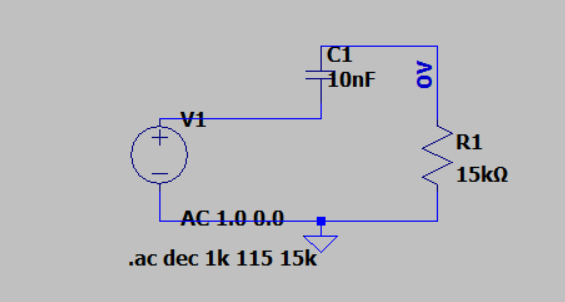
\includegraphics[scale=0.6]{./figures/CR.png}
			\caption{Κύκλωμα CR}
			\label{fig1}	
		\end{figure}
		
	Εφαρμόζοντας τον νόμο του Kirchoff για τα ρεύματα, έχουμε	
		\begin{align*}
			i_C(t) =& i_R(r)  \Rightarrow\\ 
			C\odv{(v_i-v_o)}{t}=& \frac{v_0-0}{R}\xRightarrow{v_o<<v_i}\\
			v_o = RC\odv{v_i}{t} \numberthis
		\end{align*}
	
	Άρα το CR κύκλωμα είναι διαφοριστής. Ωστόσο, χρησιμοποιήσαμε ότι $u_0 << u_i$, συνεπώς θα πρέπει να το δικαιολογήσουμε. Μετασχηματίζοντας το κύκλωματα κατά Fourier και εφαρμόζοντας τον νόμο του Kirchoff, παίρνουμε
		\begin{align*}
			\frac{V_i-V_o}{1/j\omega C} +& \frac{0-V_o}{R} = 0 \Rightarrow \\ 
			\frac{V_0}{V_i} =& H(\omega) =  \frac{Rj\omega C}{1+jR\omega C} \numberthis
				%			H(\omega) =& \frac{V_0(\omega)}{V_i(\omega)}= \frac{j+R\omega C}{1-(R\omega C)^2}R\omega C \numberthis
%			H(\omega) =& \frac{j/R\omega C + 1 }{(1/R\omega C)^2 - 1} \Rightarrow \numberthis\\
%			|H(\omega)| =& \frac{1}{|1/(R\omega C)^2 - 1|}\sqrt{1/(R\omega C)^2 + 1 } \numberthis
		\end{align*}
	Άρα έχουμε τα παρακάτω, όπου $\phi$ η διαφορά φάσης μεταξύ των δύο παλμών εισόδου-εξόδου
		\begin{align*}
			H(\omega) =& |H(\omega)| e^{j\phi}, \numberthis \\ 
				\phi =& Atan(\omega CR) \numberthis \\ 
				|H(\omega)| = & \frac{\omega CR}{1+(\omega CR)^2} \numberthis
		\end{align*}
	Παρατηρούμε ότι το κύκλωμα λειτουργεί και ως \textit{υψιπερατό φίλτρο} διότι
		\begin{itemize}
		 	\item Για \underline{\textit{$\omega\rightarrow 0$:}} $|H(\omega)|\rightarrow 0$
		 	
		 	\item Για \underline{\textit{$\omega\rightarrow\infty$:}} $|H(\omega)|\rightarrow 1$
		\end{itemize}	
	Άρα η υπόθεση $u_0 << u_i$ ισχύει στην περιοχή μικρών συχνοτήτων.
	Επίσης αν {αντιστρέψουμε} την (2) παίρνουμε τον λόγο $u_R/u_i$: 
		\begin{align*}
			h(t)=\frac{u_R}{u_i}=\delta(t) - \frac{1}{RC}e^{-t/RC}\theta(t) \numberthis
		\end{align*}
%--------------------------------------------------
\subsection*{Κύκλωμα RC}
	Τώρα θα εξετάσουμε το κύκλωμα RC. Κάνοντας τα ίδια βήματα με την προηγούμενη περίπτωση, για  $u_o<<u_i$ παίρνουμε 
		\begin{figure}[h!]
			\centering 
			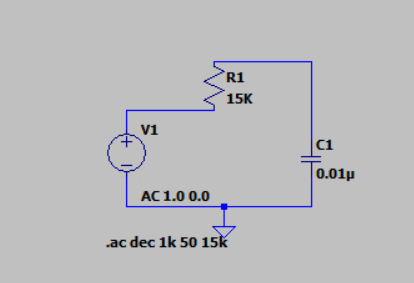
\includegraphics[scale=0.6]{./figures/RC.png}
			\caption{Κύκλωμα RC}
			\label{fig2}
		\end{figure}
	
		\begin{align*}
				u_0(t) = \frac{1}{RC}\int_{0}^{t'} v_i(t') dt' \numberthis
		\end{align*}
	Άρα το εν λόγω κύκλωμα είναι ολοκληρωτής του σήματος εισόδου. Μετασχηματίζοντας πάλι κατά Fourier, παίρνουμε τα παρακάτω αποτελέσματα
		\begin{align*}
			H(\omega) =& \frac{1}{j\omega RC + 1 }  = |H(\omega)| e^{j\phi}\numberthis\\
			|H(\omega)| =& \frac{1}{\sqrt{1+(\omega RC)^2}} \numberthis\\
			\phi        =& -Arctan(\omega CR)\numberthis
		\end{align*}
	Παρατηρούμε ότι το κύκλωμα λειτουργεί και ως \textit{βαθυπερατό φίλτρο}, διότι
		\begin{itemize}
			\item \underline{\textit{Για $\omega\rightarrow0$}}:$|H(\omega)| \rightarrow 1$
			
			\item \underline{\textit{Για $\omega\rightarrow\infty$}}: $|H(\omega)| \rightarrow 0$
		\end{itemize}	
	Τέλος, αντιστρέφοντας την (6), βρίσκουμε την σχέση των πλατών των δύο σημάτων: 
	\begin{align*}
		h(t) = \frac{u_C}{u_i} = \frac{1}{RC}e^{-t/RC}\theta(t) \numberthis
	\end{align*}
	
\section*{Πειραματικά Δεδομένα \& Ανάλυση} 
	\subsection*{Κύκλωμα CR} 
		Για την πειραματική μελέτη των κυκλωμάτων, θέλουμε να δούμε την απόκριση της εξόδου συναρτήσει της συχνότητας του σήματος εισόδου. Συγκεκριμένα θα εξετάσουμε πως συμπεριφέρονται για μεταβαλλόμενες τιμές της συχνότητας για αρμονικούς παλμούς εισόδου, δηλαδή θα εξετάσουμε την ιδιότητά τους να λειτουργούν ως φίλτρα και επιπλέον βάζοντας παλμούς διαφορετικής μορφής θα εξετάσουμε πώς αυτή μεταβάλλεται.
		
		Ξεκινώντας την μελέτη των ιδιοτήτων περί συχνότητας, θα έχουμε ως είσοδο έναν παλμό πλάτους $u_i = 2V$ και για τιμές συχνότητας στο φάσμα $f=115Hz-15kHz$ θα μετράμε τόσο το πλάτος του σήματος εξόδου όσο και την χρονική διαφορά μεταξύ εισόδου-εξόδου για να μπορέσουμε εν τέλει να βρούμε την διαφορά φάσης τους. Έτσι θα ελέγξουμε πειραματικά τις σχέσεις (4) και (5). 
		
		Οι μετρήσεις και άλλα μεγέθη που προκύπτουν από αυτές φαίνονται στον Πίνακα (\ref{tab1}).
		
		\begin{table}
			\centering
			\begin{tabular}{c|c|c||c|c|}
			$f(Hz)$ & $u_R/u_i(V)$ & $\Delta t(\mu s)$ & $A_{db}(db)$ & $\phi(rad)$ \\
			\hline\hline
			115 & $0.11 \pm 0.01$ & $1200.00 \pm 20.00$ & $-9.59 \pm 0.43$ & $0.87 \pm 0.01$\\
170 & $0.15 \pm 0.02$ & $1200.00 \pm 20.00$ & $-8.24 \pm 0.43$ & $1.28 \pm 0.02$\\
250 & $0.23 \pm 0.02$ & $800.00 \pm 10.00$ & $-6.38 \pm 0.43$ & $1.26 \pm 0.02$\\
400 & $0.32 \pm 0.03$ & $400.00 \pm 5.00$ & $-4.95 \pm 0.43$ & $1.01 \pm 0.01$\\
600 & $0.42 \pm 0.04$ & $250.00 \pm 5.00$ & $-3.77 \pm 0.43$ & $0.94 \pm 0.02$\\
850 & $0.60 \pm 0.06$ & $180.00 \pm 1.00$ & $-2.22 \pm 0.43$ & $0.96 \pm 0.01$\\
1300 & $0.75 \pm 0.08$ & $90.00 \pm 1.00$ & $-1.25 \pm 0.43$ & $0.74 \pm 0.01$\\
2000 & $0.85 \pm 0.09$ & $30.00 \pm 0.50$ & $-0.71 \pm 0.43$ & $0.38 \pm 0.01$\\
3000 & $0.90 \pm 0.09$ & $20.00 \pm 0.20$ & $-0.46 \pm 0.43$ & $0.38 \pm 0.00$\\
4500 & $0.97 \pm 0.10$ & $10.00 \pm 0.10$ & $-0.11 \pm 0.43$ & $0.28 \pm 0.00$\\
6500 & $0.97 \pm 0.10$ & $6.00 \pm 0.10$ & $-0.11 \pm 0.43$ & $0.25 \pm 0.00$\\
10000 & $0.97 \pm 0.10$ & $3.00 \pm 0.05$ & $-0.11 \pm 0.43$ & $0.19 \pm 0.00$\\
15000 & $0.97 \pm 0.10$ & $1.50 \pm 0.05$ & $-0.11 \pm 0.43$ & $0.14 \pm 0.00$
			\end{tabular}
			\caption{Πειραματικές Μετρήσεις}
			\label{tab1}
		\end{table}
	\newpage
		

		Στις Εικόνες (\ref{fig3}), (\ref{fig4}), (\ref{fig5}), φαίνονται οι γραφικές παραστάσεις $u_R/u_i - f$, $A_{db} - f$, $\phi - f$ αντίστοιχα. Σε κάθε μία από αυτές υπάρχουν τα πειραματικά σημεία και οι καμπύλες από την θεωρία, το fitting και την προσομοίωση μέσω LTSpice. 
		Η συχνότητα μισής ισχύος προκύπτει γραφικά από την προσαρμοσμένη καμπύλη στα δεδομένα $A_{db}$ και είναι ίση με $f_b = (665\pm 1)Hz$.
		\begin{figure}[h!]
			\centering 
			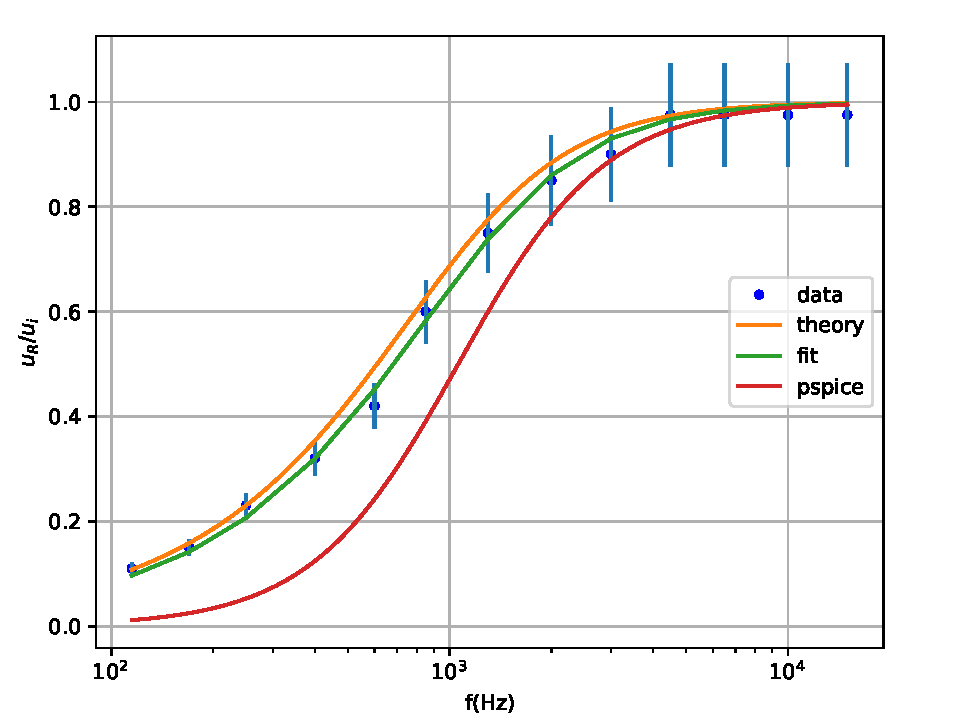
\includegraphics[scale=0.7]{../plots/CR_f-Ur.pdf}
			\caption{$u_R/u_i - f$. Η θεωρητική καμπύλη δίνεται από την (5)}
			\label{fig3}
		\end{figure}
		
		\begin{figure}[h!]
			\centering 
			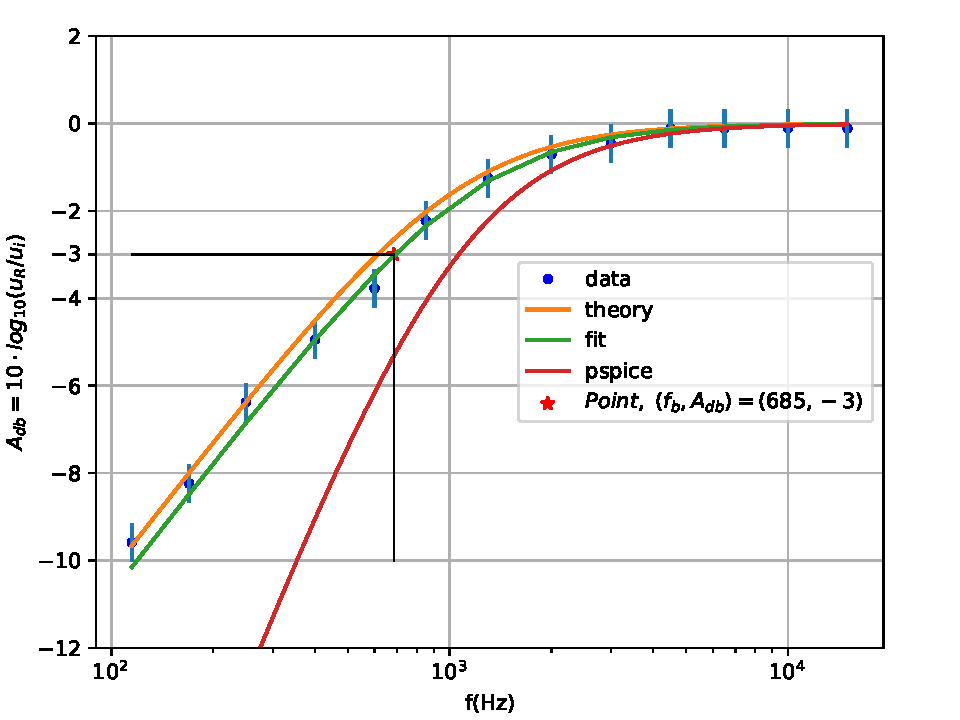
\includegraphics[scale=0.7]{../plots/CR_f-Adb.pdf}
			\caption{$A_{db} - f$. Φαίνεται και η συχνότητα μισής ισχύος που αντιστοιχεί στα -3db. Η θεωρητική καμπύλη δίνεται από την (5) και συγκεκριμένα είναι $A_{db}=10log(u_R/u_i)$}
			\label{fig4}
		\end{figure}
		
		\begin{figure}[h!]
			\centering 
			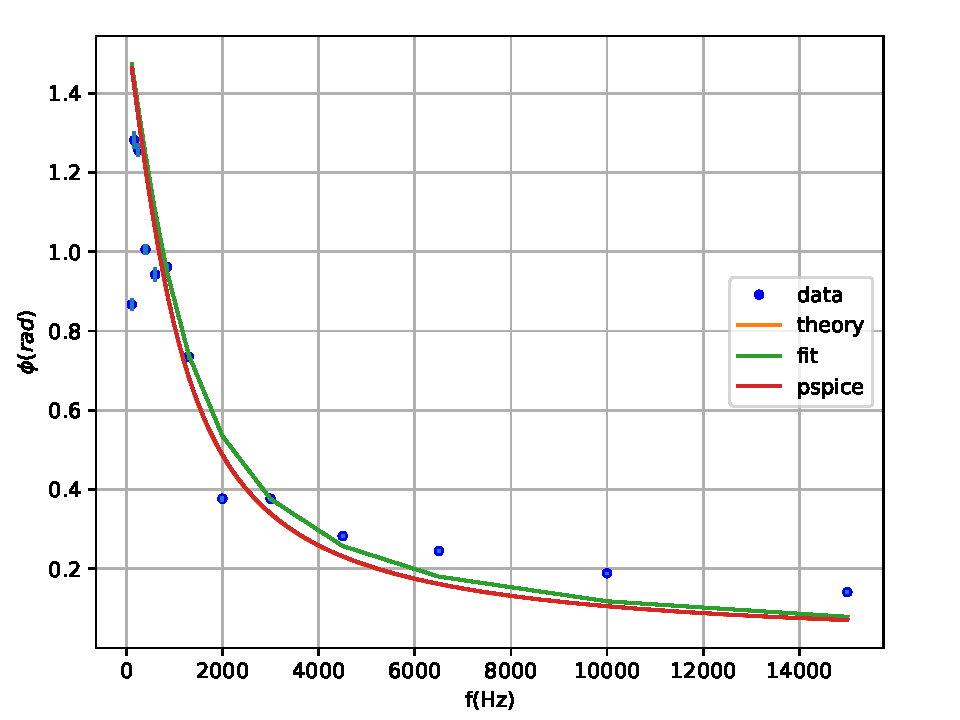
\includegraphics[scale=0.7]{../plots/CR_f-phi.pdf}
			\caption{$\phi - f$. Η θεωρητική καμπύλη δίνεται από την (4)}
			\label{fig5}
		\end{figure}
		
		
			
	Τέλος, βλέπουμε την ασυμπτωτική συμπεριφορά του CR κυκλώματος, για $f >> f_b = 685$ στην παρακάτω Εικόνα (\ref{fig6}). Από γραμμική προσαρμογή προκύπτει η ευθεία $y= 1.81\times10^{-5} x + -0.32$, η οποία είναι σχεδόν οριζόντια, όπως αναμέναμε.
	
		\begin{figure}[h!]
			\centering 
			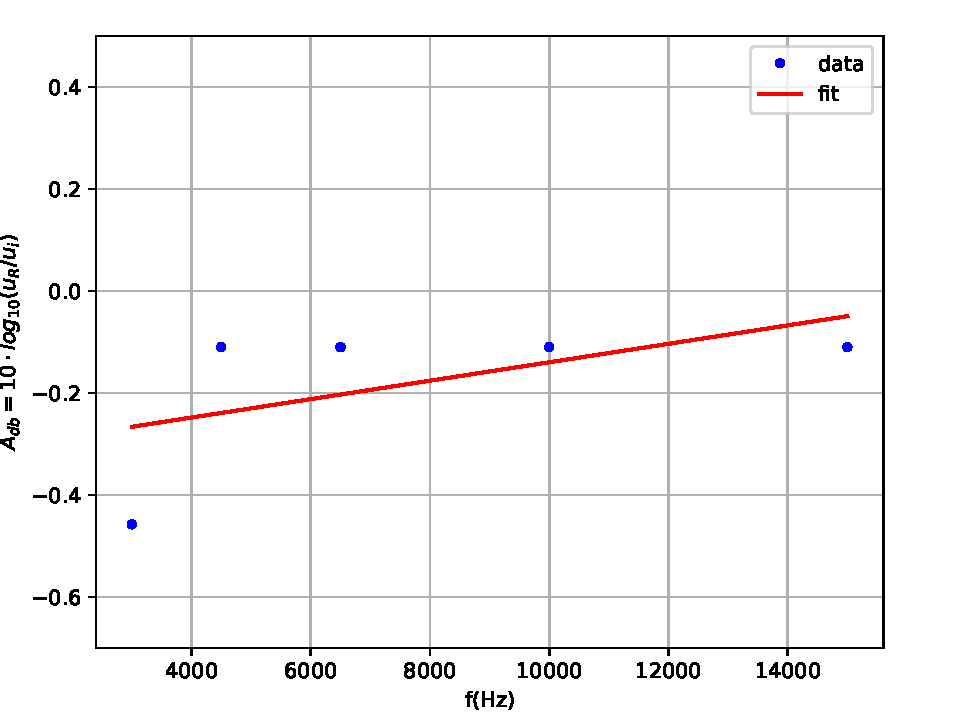
\includegraphics[scale=0.7]{../plots/CR_f-Adb-linear.pdf}
			\caption{Ασυμπτωτική Συμπεριφορά του CR}
			\label{fig6}
		\end{figure}
	
\newpage	
		
	\subsubsection*{Μελέτη CR ως διαφοριστή}
		Θα εισάγουμε δύο διαφορετικούς παλμούς, έναν τετραγωνικό και έναν τριγωνικό συχνότητας 1kHz και πλάτους 1V. Η προσομοίωση με το LTSpice φαίνεται στις παρακάτω Εικόνες (\ref{fig7}) και (\ref{fig8}) και τα ποιοτικά αποτελέσματα είναι ίδια με τα πειραματικά 
			\begin{figure}[h!]
				\centering 
				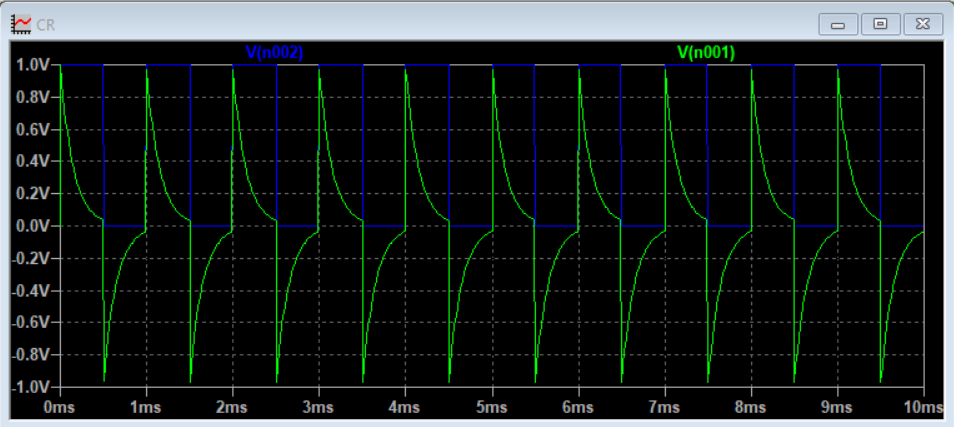
\includegraphics[scale=0.4]{./figures/cr_rec.png}
				\caption{Εισαγωγή τετραγωνικού παλμού στο CR, $f=1kHZ$.}
				\label{fig7}
			\end{figure}
		
		\begin{figure}[h!]
			\centering 
			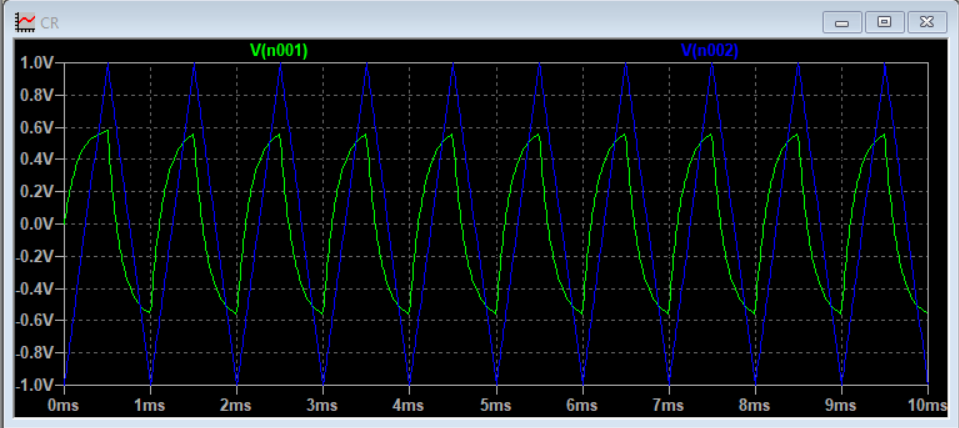
\includegraphics[scale=0.4]{./figures/cr_triag.png}
			\caption{Εισαγωγή τριγωνικού παλμού στο CR, $f=1kHZ$.}
			\label{fig8}
		\end{figure}
		
\newpage		
		
	Παρατηρούμε πως το σήμα εξόδου δεν είναι ακριβώς η παράγωγος του σήματος εισόδου, διότι η σχέση στην οποία βασιστήκαμε για να πούμε πως το CR είναι διαφοριστής είναι προσεγγιστική.	
	Άρα περιμένουμε αν μειώσουμε την συχνότητα ο χαρακτήρας του κυκλώματος ως διαφοριστή να γίνει εμφανέστερος. Ωστόσο, επειδή το κύκλωμα δρα και ως βαθυπερατό φίλτρο, θα έχουμε πολύ πολυ μικρότερο πλάτος. Όλα αυτά διαπιστώνονται και στις παρακάτω Εικόνες (\ref{fig9}) και (\ref{fig10}), όπου οι παλμοί είναι συνχότητας 10kHz
		
		\begin{figure}[h!]
			\centering 
			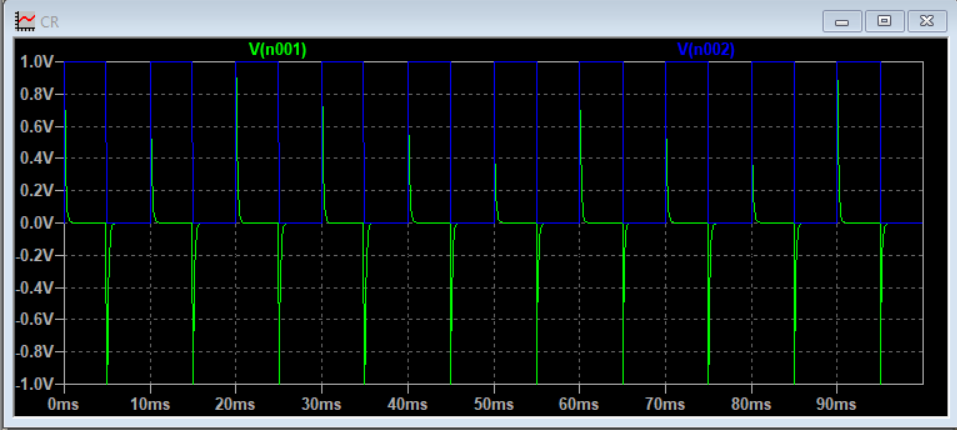
\includegraphics[scale=0.4]{./figures/cr_rec_10.png}
			\caption{Εισαγωγή τετραγωνικού παλμού στο CR, $f=10kHZ$.}
			\label{fig9}
		\end{figure}
		
		\begin{figure}[h!]
			\centering 
			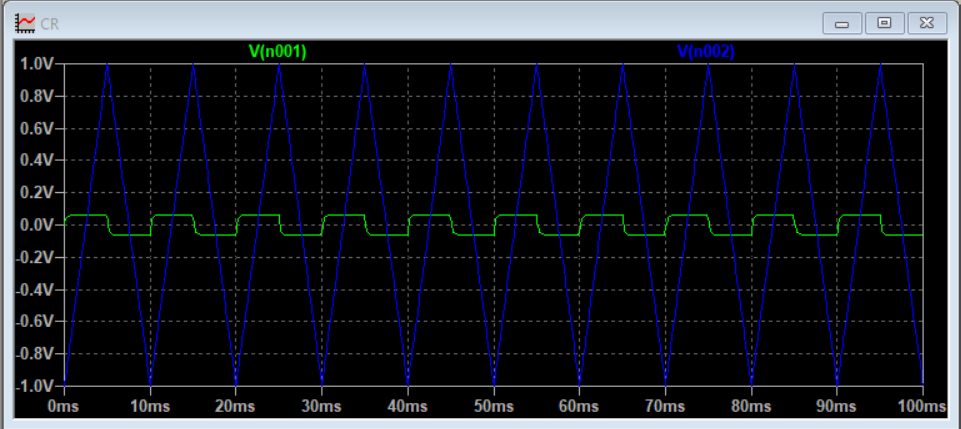
\includegraphics[scale=0.4]{./figures/cr_triag_10.png}
			\caption{Εισαγωγή τριγωνικού παλμού στο CR, $f=10kHZ$.}
			\label{fig10}
		\end{figure}
		
		\newpage
		
%---------------------------------------------------------------		
	\subsection*{Κύκλωμα RC}
		Παρόμοια με πριν θα εξετάσουμε τις περί συχνότητας ιδιότητες του κυκλώματος, θεωρώντας πάλι παλμό $u_i = 2V$ και τιμές συχνότητας στο φάσμα $f=50Hz-15kHz$. Θα ελέγξουμε δηλαδή τις σχέσεις (9) και (10)
		Οι πειραματικές μετρήσεις και κάποια παράγωγα μεγέθη φαίνονται στον Πίνακα (\ref{tab2})
		
		\begin{table}[h!]
			\centering
			\begin{tabular}{c|c|c||c|c|}
			$f(Hz)$ & $u_R/u_i(V)$ & $\Delta t(\mu s)$ & $A_{db}(db)$ & $\phi(rad)$ \\
			\hline\hline
50 & $0.97 \pm 0.10$ & $700.00 \pm 20.00$ & $-0.11 \pm 0.43$ & $0.22 \pm 0.01$\\
75 & $0.97 \pm 0.10$ & $400.00 \pm 20.00$ & $-0.11 \pm 0.43$ & $0.19 \pm 0.01$\\
115 & $0.97 \pm 0.10$ & $300.00 \pm 10.00$ & $-0.11 \pm 0.43$ & $0.22 \pm 0.01$\\
170 & $0.95 \pm 0.10$ & $200.00 \pm 10.00$ & $-0.22 \pm 0.43$ & $0.21 \pm 0.01$\\
250 & $0.95 \pm 0.10$ & $200.00 \pm 5.00$ & $-0.22 \pm 0.43$ & $0.31 \pm 0.01$\\
400 & $0.90 \pm 0.09$ & $200.00 \pm 5.00$ & $-0.46 \pm 0.43$ & $0.50 \pm 0.01$\\
600 & $0.85 \pm 0.09$ & $160.00 \pm 2.00$ & $-0.71 \pm 0.43$ & $0.60 \pm 0.01$\\
850 & $0.75 \pm 0.08$ & $140.00 \pm 2.00$ & $-1.25 \pm 0.43$ & $0.75 \pm 0.01$\\
1300 & $0.61 \pm 0.06$ & $120.00 \pm 1.00$ & $-2.15 \pm 0.43$ & $0.98 \pm 0.01$\\
2000 & $0.45 \pm 0.05$ & $90.00 \pm 0.50$ & $-3.47 \pm 0.43$ & $1.13 \pm 0.01$\\
3000 & $0.31 \pm 0.03$ & $70.00 \pm 0.50$ & $-5.09 \pm 0.43$ & $1.32 \pm 0.01$\\
4500 & $0.22 \pm 0.02$ & $45.00 \pm 0.50$ & $-6.58 \pm 0.43$ & $1.27 \pm 0.01$\\
6500 & $0.15 \pm 0.02$ & $35.00 \pm 0.50$ & $-8.10 \pm 0.43$ & $1.43 \pm 0.02$\\
10000 & $0.10 \pm 0.01$ & $20.00 \pm 0.20$ & $-10.00 \pm 0.43$ & $ 1.26 \pm 0.01$\\
15000 & $0.07 \pm 0.01$ & $14.00 \pm 0.10$ & $-11.55 \pm 0.44$ & $ 1.32 \pm 0.01$
			\end{tabular}
			\caption{Πειραματικές Μετρήσεις}
			\label{tab2}
		\end{table}		

\newpage

Στις Εικόνες (\ref{fig11}), (\ref{fig12}), (\ref{fig13}), φαίνονται οι γραφικές παραστάσεις $u_R/u_i - f$, $A_{db} - f$, $\phi - f$ αντίστοιχα. Σε κάθε μία από αυτές υπάρχουν τα πειραματικά σημεία και οι καμπύλες από την θεωρία, το fitting και την προσομοίωση μέσω LTSpice. 
		Η συχνότητα μισής ισχύος προκύπτει γραφικά από την καμπύλη που έχω κάνει fit στα δεδομένα και είναι ίση με $f_b = (1671\pm 5)Hz$.

		
		\begin{figure}[h!]
			\centering 
			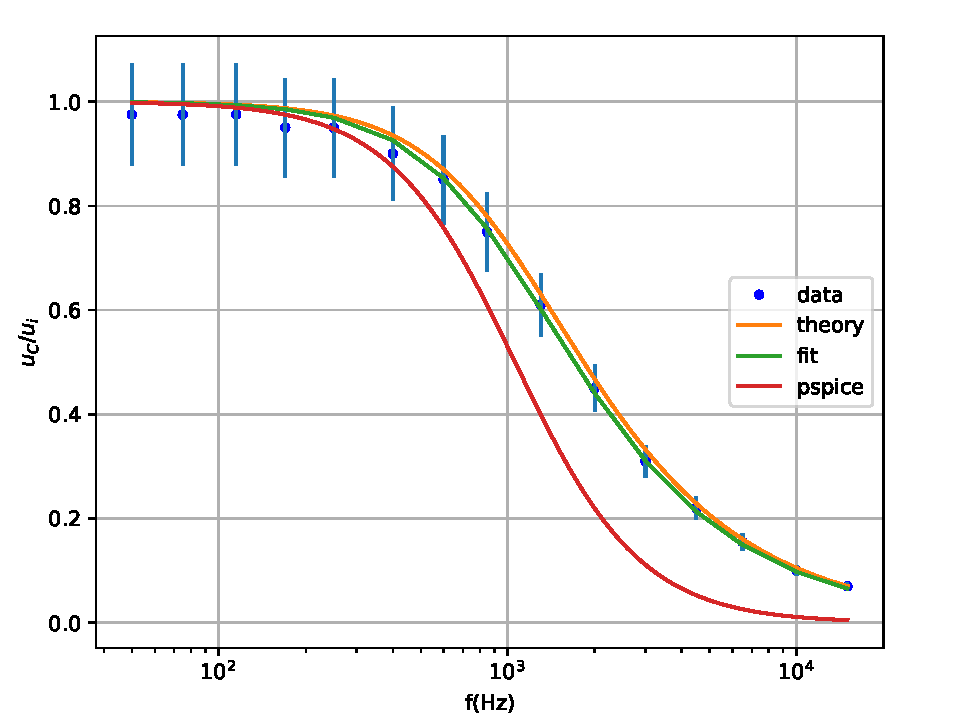
\includegraphics[scale=0.7]{../plots/RC_f-Uc.pdf}
			\caption{$u_R/u_i - f$. Η θεωρητική καμπύλη δίνεται από την (9)}
			\label{fig11}
		\end{figure}
		
				\begin{figure}[h!]
			\centering 
			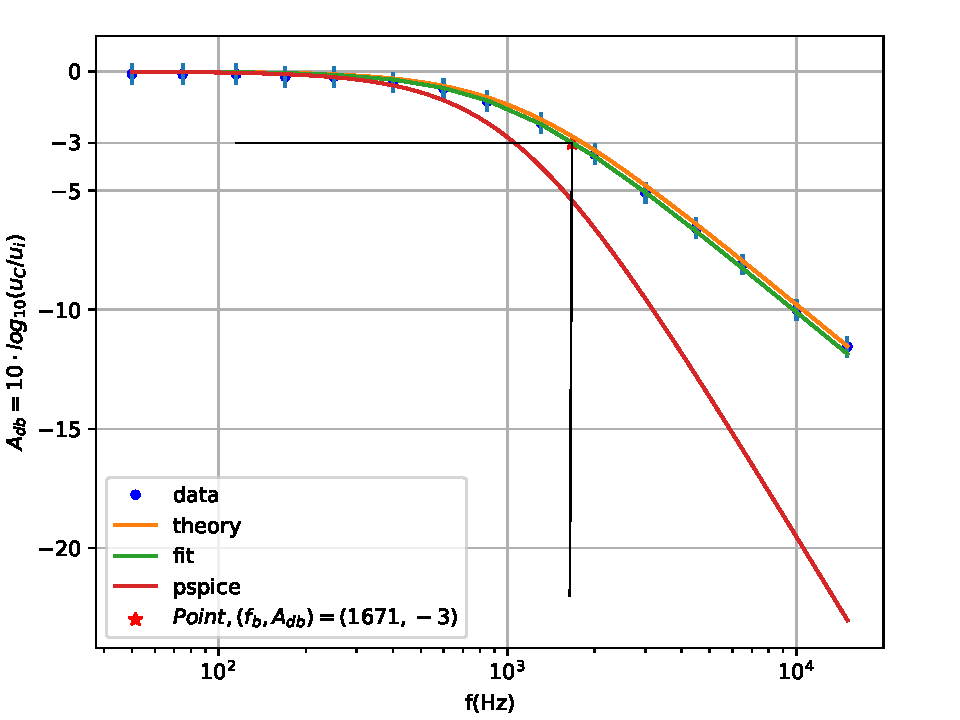
\includegraphics[scale=0.7]{../plots/RC_f-Adb.pdf}
			\caption{$A_{db} - f$. Φαίνεται και η συχνότητα μισής ισχύος που αντιστοιχεί στα -3db. Η θεωρητική καμπύλη προκύπτει από την (9) και συγκεκριμένα είναι $A_{db}=10log_{10}(u_C/u_i)$.}
			\label{fig12}
		\end{figure}
		
		\begin{figure}[h!]
			\centering 
			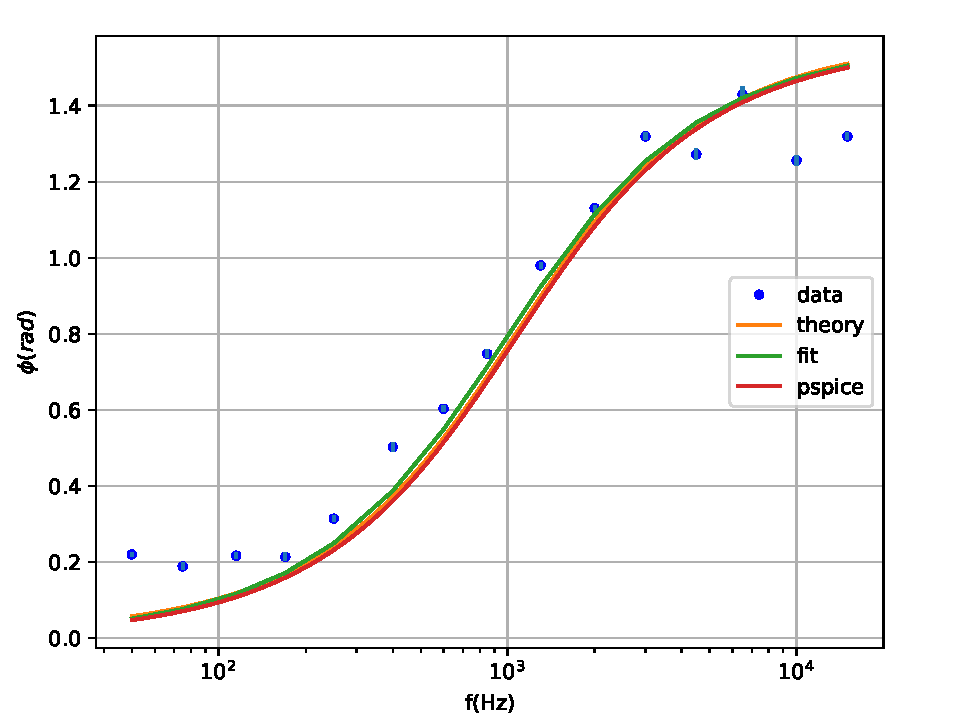
\includegraphics[scale=0.7]{../plots/RC_f-phi.pdf}
			\caption{$\phi - f$. Η θεωρητική καμπύλη δίνεται από την (10)}
			\label{fig13}
		\end{figure}	
		
		Τέλος, βλέπουμε την ασυμπτωτική συμπεριφορά του RC κυκλώματος, για $f << f_b = 1671Hz$ στην παρακάτω Εικόνα (\ref{fig14}). Από γραμμική προσαρμογή προκύπτει η ευθεία $y= 6.87\times10^{-4} x + -0.06$, η οποία είναι σχεδόν οριζόντια, όπως αναμέναμε.
	
		\begin{figure}[h!]
			\centering 
			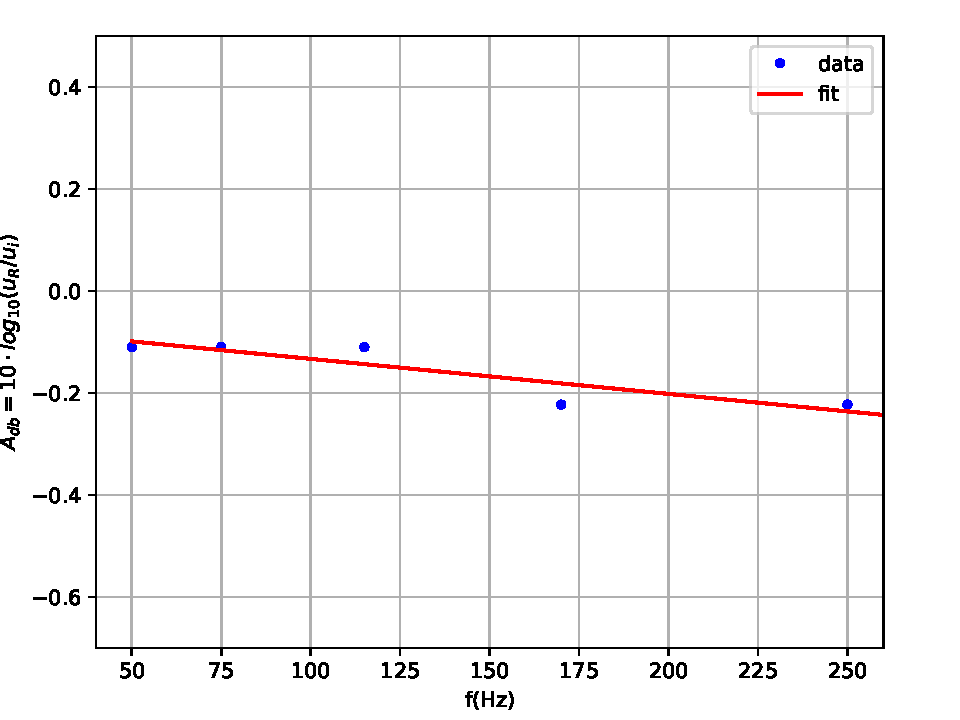
\includegraphics[scale=0.7]{../plots/RC_f-Adb-linear.pdf}
			\caption{Ασυμπτωτική Συμπεριφορά του RC, για $f << f_b = 1671Hz$}
			\label{fig14}
		\end{figure}	
		
		\newpage
		
		
		\subsubsection*{Μελέτη RC ως ολοκληρωτή}
		Θα εισάγουμε δύο διαφορετικούς παλμούς, έναν τετραγωνικό και έναν τριγωνικό συχνότητας 1kHz και πλάτους 1V. Η προσομοίωση με το LTSpice φαίνεται στις παρακάτω Εικόνες (\ref{fig15}) και (\ref{fig16}) και τα ποιοτικά αποτελέσματα είναι ίδια με τα πειραματικά 
	\newpage
			\begin{figure}[h!]
				\centering 
				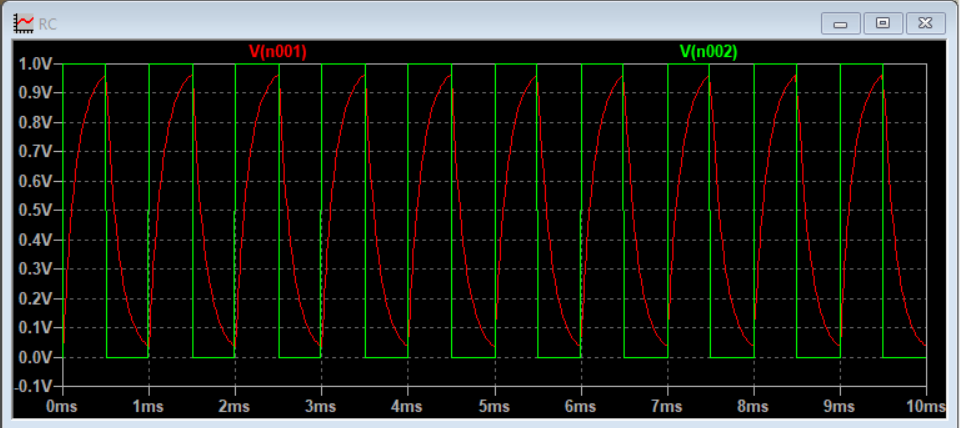
\includegraphics[scale=0.4]{./figures/rc_rec.png}
				\caption{Εισαγωγή τετραγωνικού παλμού στο RC, $f=1kHZ$.}
				\label{fig15}
			\end{figure}
		
		\begin{figure}[h!]
			\centering 
			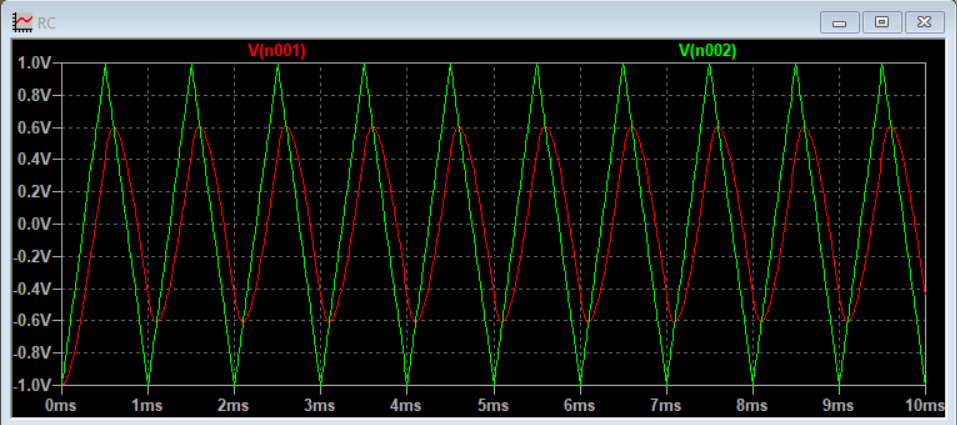
\includegraphics[scale=0.4]{./figures/rc_triag.png}
			\caption{Εισαγωγή τριγωνικού παλμού στο RC, $f=1kHZ$.}
			\label{fig16}
		\end{figure}
	
	
\section*{Σύγκριση με Προσομοιώσεις}
	Παρατηρούμε πως στις προσομοιώσεις οι καμπύλες των φάσεων συμπίπτουν ακριβώς με τις πειραματικές. Ωστόσο οι καμπύλες των πλατών δεν συμπίπτουν. Κατά πάσα πιθανότητα αυτό οφείλεται σε λανθασμένες ρυθμίσεις στο LTspice τις οποίες δεν κατάφερα να βρω και να διορθώσω.
	
\section*{Συμπεράσματα}
	Τα πειραματικά με θεωρητικά δεδομένα συμπίπτουν στα όρια του σφάλματος. Η προσομοίωση με το LTSpice δίνει σωστά ποιοτικά αποτελέσματα αλλά ο λόγος των πλατών των σημάτων εισόδου/εξόδου δεν συμπίπτει με τα δεδομένα του πειράματος, λογικά εξαιτίας κάποιων παραμέτρων τις οποίες δεν κατάφερα να βρω.

\end{document}